\section{BBSim: An Event Driven Simulator for Burst Buffer}
\label{Sec:Simulation}

We develop an event-driven simulator, named \textbf{BBSim},
to simulate how Cerberus schedules jobs on burst-buffer-enabled HPC systems.
Apart from demonstrating the lifetime of a job scheduled by Cerberus,
Figure~\ref{Fig:JobFSM} also illustrates the various events in BBSim and how to handle
them in an event-driven-simulation approach.
The transitions of job \textit{state}, along with which an \textit{action} is triggered,
depend on the current state and the \textit{event} happened.
For example, when $job_i$ is submitted to the system,
it enters the \textit{Waiting Stage-in} state,
waiting to be scheduled in the job queue $Q_I$. 
The scheduler checks $job_i$'s resource demand and
dispatches it to run when sufficient resources are available.

Various \texttt{release()} actions are important because, in addition to job submissions,
\texttt{schedule()} will be invoked to schedule the waiting jobs.
The allocated resource can only be released when one phase is finished.
Therefore, any \textit{dispatch} event, generated by the \texttt{schedule()} action,
follows a certain \textit{finish} event.
The allocated resources are released at the following time points:
\begin{itemize}
        \item When $job_i$ pre-fetches data from the burst buffer to the memory,
                the burst buffer allocated in the stage-in phase ($BB_{in}$) is released.
        \item When $job_i$ completes the computation,
                the system reclaims the burst buffer allocated in the running phase ($BB_{run}$).
        \item When $job_i$ output data is written to the burst buffer from the memory,
              compute nodes ($CN$) allocated in the running phase are released.
        \item When output data are drained out to the external storage,
                the burst buffer allocated in the stage-out phase ($BB_{out}$) is released.
                The simulation for $job_i$ completes.
\end{itemize}

% Notice that resource can only be released when certain phase is finished.
% Therefore, any \textit{dispatch} event, caused by \texttt{schedule()} action, actually happens
% at the meanwhile of a certain \textit{finish} event.
% The timestamps of all possible \textit{finish} events are calculated in the following way:
% \begin{align}
%         & TS_{f\_stagein} = TS_{s\_stagein} + \frac{bb\_in}{BW_{io\_to\_bb}}\label{Equ:FinIn} \\
%         & TS_{f\_loadin} = TS_{s\_run} + \frac{bb\_in}{BW_{bb\_to\_cn}}\label{Equ:FinMemIn} \\
%         & TS_{f\_run} = TS_{f\_loadin} + \frac{bb\_run}{BW_{cn\_to\_bb}} + rt\label{Equ:FinRun} \\
%         & TS_{f\_loadout} = TS_{s\_stageout} + \frac{bb\_out}{BW_{cn\_to\_bb}}\label{Equ:FinMemOut} \\
%         & TS_{f\_stageout} = TS_{f\_loadout} + \frac{bb\_out}{BW_{bb\_to\_io}} \label{Equ:FinOut}
% \end{align}
% where $TS_{f\_x}$ stands for the timestamps of finishing phase $x$,
% $TS_{s\_x}$ stands for the timestamps of starting phase $x$,
% $BW_{x\_to\_y}$ stands for the bandwidth between $x$ and $y$.
% 
% Though target on burst buffer system, BBSim also supports simulating non-BB HPC system.
% Besides, it is not coupled with Cerberus but easy to simulating many other scheduler.
% Both can be proved by the following experiments for various schedulers.


%The timestamps of all the \textit{finish} events are calculated as follows:
%\begin{align}
%        & TS_{f\_stagein} = TS_{s\_stagein} + \frac{bb\_in}{BW_{io\_to\_bb}}\label{Equ:FinIn} \\
%        & TS_{f\_loadin} = TS_{s\_run} + \frac{bb\_in}{BW_{bb\_to\_cn}}\label{Equ:FinMemIn} \\
%        & TS_{f\_run} = TS_{f\_loadin} + \frac{bb\_run}{BW_{cn\_to\_bb}} + rt\label{Equ:FinRun} \\
%        & TS_{f\_loadout} = TS_{s\_stageout} + \frac{bb\_out}{BW_{cn\_to\_bb}}\label{Equ:FinMemOut} \\
%        & TS_{f\_stageout} = TS_{f\_loadout} + \frac{bb\_out}{BW_{bb\_to\_io}} \label{Equ:FinOut}
%\end{align}
%where $TS_{f\_x}$ stands for the timestamps of the finishing phase $x$,
%$TS_{s\_x}$ stands for the timestamps of the starting phase $x$,
%$BW_{x\_to\_y}$ stands for the bandwidth between $x$ and $y$.
%BBSim does not simulate the data transfer between I/O nodes and PFS through the network.

% % system
% We consider simulating the full Trinity super computer\cite{TrinitySystem}.
% The number of compute nodes on Trinity is about 18,936,
% e.g. 9,436 Intel Haswell nodes
% and at least 9500 Intel Xeon Phi nodes.
% There are 16 cores on each processor, thus totally 302,976 cores.
% In the following experiments, we compare two identical system except that
% I/O nodes are replaced by the same number of burst buffer nodes.
% Eventually Trinity plans to delivery up to 576 burst buffer nodes of 3.7 PB,
% consisted of Trinity I/O nodes with PCIe SSD card.
% They are globally accessible as intermediate storage and distributed among cabinets.
% Sequential read/write speed of burst buffer nodes is 8.0 GBps.
% Bandwidth between CPU node and non-burst-buffer I/O node is set to 2.5 GBps.


Our Python implementation of BBSim includes three major modules.
The \texttt{simulator} module drives the event-driven simulation process.
Various job models, job demands, and schedulers are in \texttt{scheduler} module.
The \texttt{dp\_solver} module provides dynamic programming solutions for
the \texttt{Cerberus} scheduler in \texttt{scheduler}.
Though targeting on burst buffer enabled systems,
BBSim also supports simulating job scheduling on HPC systems without burst buffer.
Besides, it is easy to integrate other scheduling policies into BBSim.
For example, we have implemented the naive burst-buffer aware scheduler
(e.g. SLURM shown in Figure~\ref{Fig:SlurmQueue}) as a scheduling module in BBSim,
which enable us to evaluate the performance improvement achieved by our multiple-queue Cerberus.
The codebase of BBSim and Cerberus will be made public to the community.

We use BBSim to simulate
a burst-buffer-enabled HPC system shown in Figure~\ref{Fig:BBArchitecture}.
The system adopts traditional IBM Blue Gene/P architecture but burst buffer are
assumably available in the I/O nodes.
The system consists of 18,936 compute nodes,
e.g., 9,436 Intel Haswell nodes and 9,500 Intel Xeon Phi nodes.
The parameters related to burst buffer are taken from the 
NERSC-8 Use Case Scenarios technical report\cite{BBUseCase} on Trinity system\cite{TrinitySystem},
the next generation supercomputer in Los Alamos National Laboratory.
Specifically, there are 576 burst buffer enabled nodes with aggregated 3.7 PB storage,
which are globally accessible as the intermediate storage.
The sequential read/write speed of burst buffer nodes is 8.0 GBps.
The bandwidth between a CPU node and an I/O node is set to 2.5 GBps.
The time spent for job's I/O operation in our simulation is calculated by
dividing the amount of transferred data by the corresponding bandwidth.

\begin{figure}[htp]
        \centering
        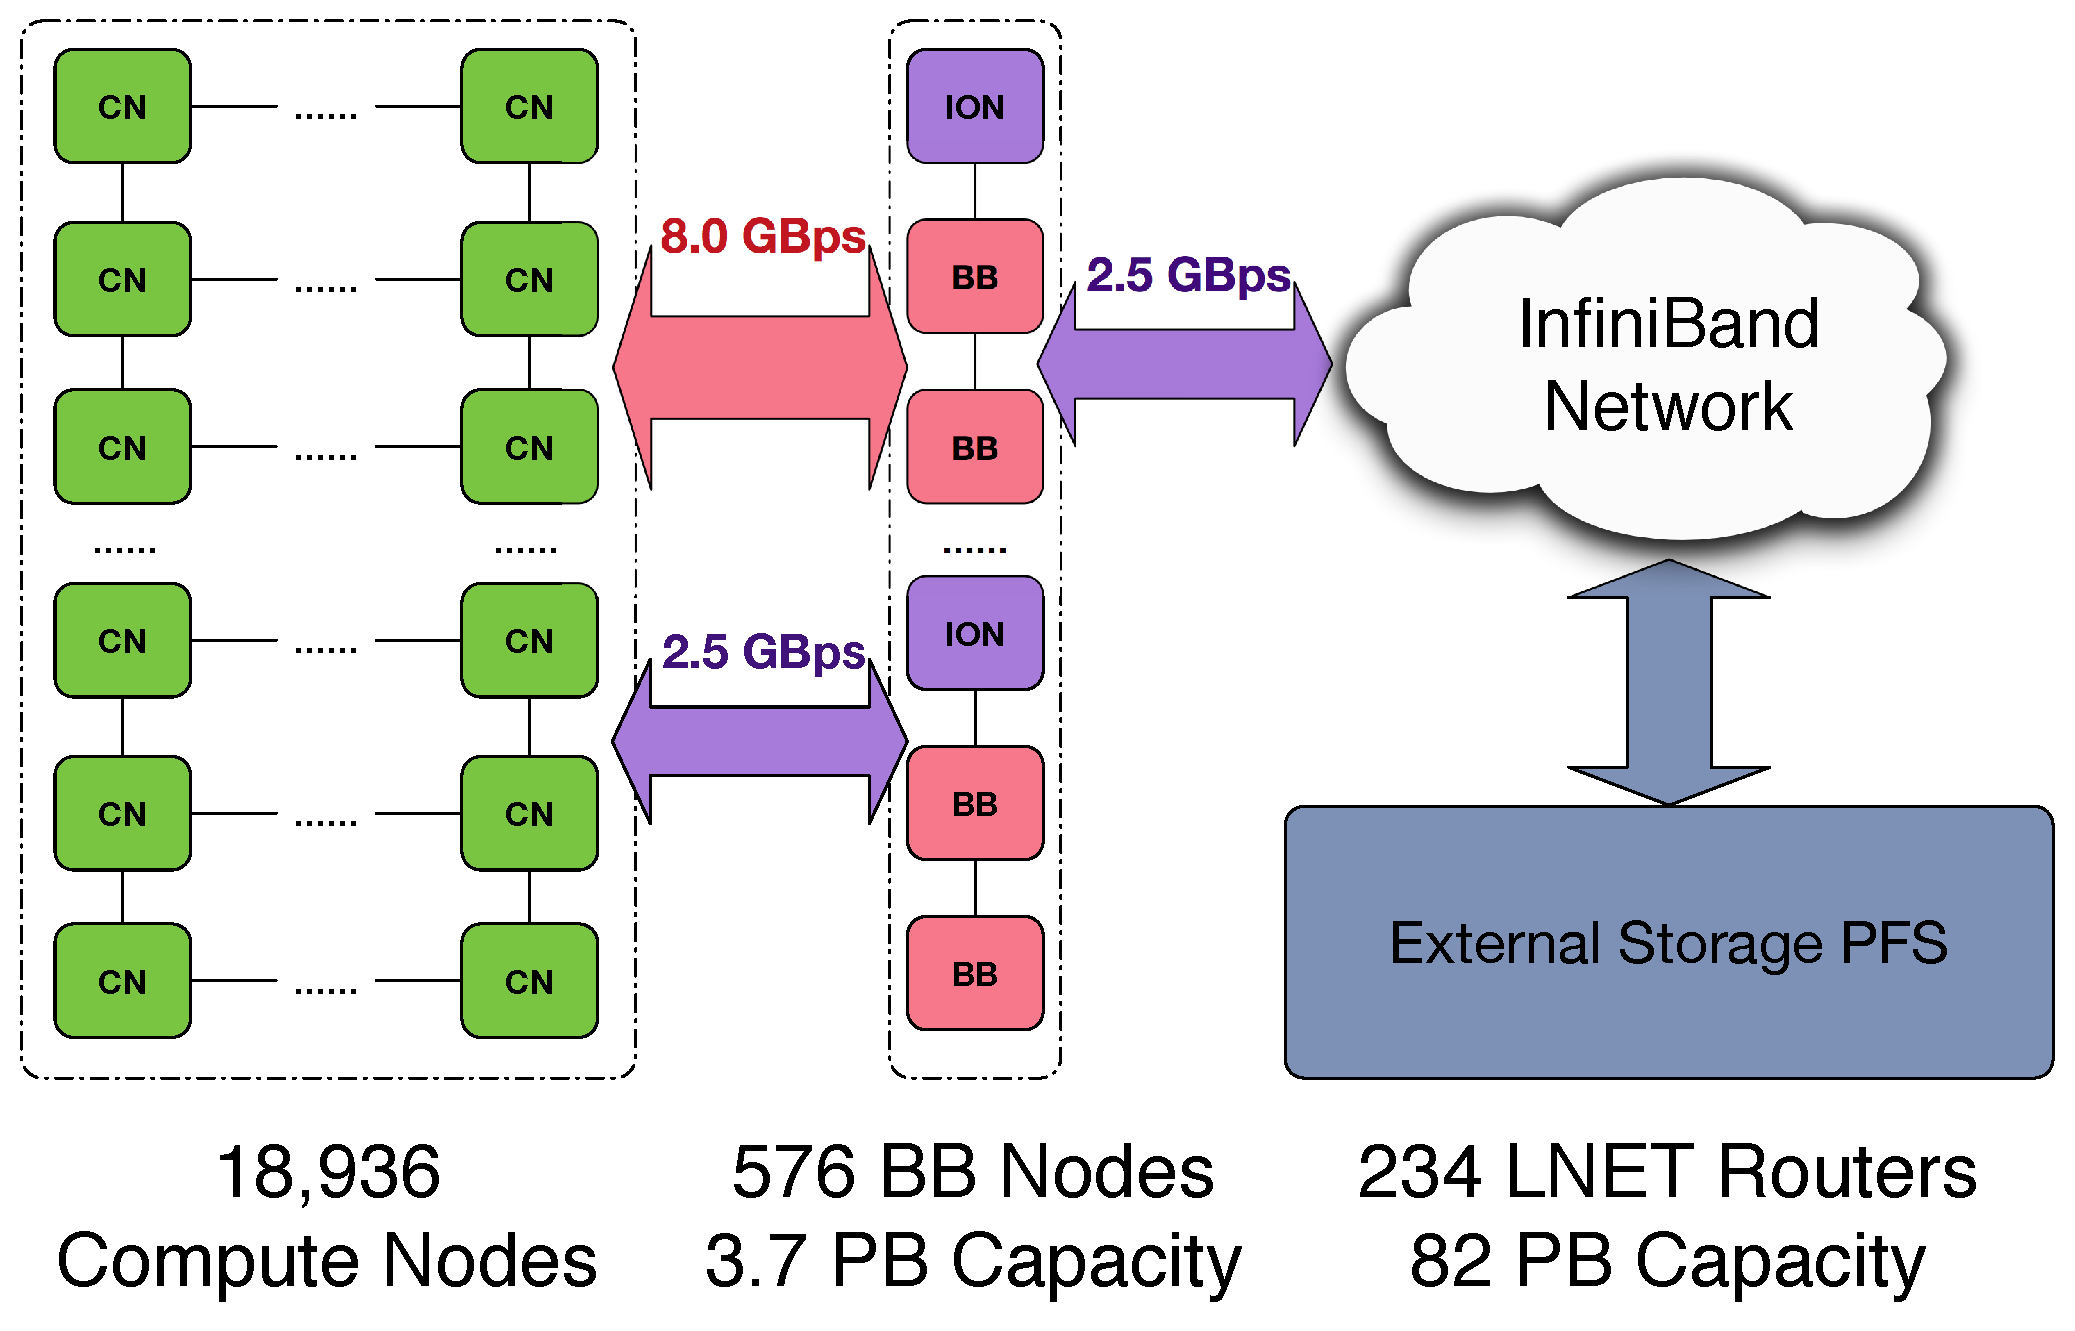
\includegraphics[width=3.5in]{BBArchitecturewithBandwidth}
        \caption{A burst buffer enabled system simulated in BBSim. The bandwidth between compute nodes and burst buffer node is 8.0 GBps (denoted by red arrow). The bandwidth between compute nodes and I/O nodes, and the bandwidth between I/O layer and the outside InfiniBand Network are set to 2.5 GBps (denoted by purple arrow).}
\label{Fig:BBArchitecture}
\end{figure}

